\documentclass[master=cws,masteroption=vs,english]{kulemt}

\setup{	title={OBD\textendash II Access Control},
		author={Michiel Willems},
		promotor={Prof. dr. Bruno Crispo},
		assessor={test},
		assistant={test}}

\usepackage{graphicx}
\usepackage{fixltx2e}
\usepackage{csquotes}
\usepackage{epigraph}
\usepackage{mathtools}
\usepackage[table,xcdraw]{xcolor}
\usepackage[hang]{footmisc}
\usepackage{cryptocode}
\usepackage{url}
\usepackage[pdfusetitle,colorlinks,plainpages=false]{hyperref}
\usepackage[numbers]{natbib}
\setlength\footnotemargin{1em}
\graphicspath{ {images-thesis/} }

\setup{	filingcard,
		translatedtitle={Beste masterproef ooit al geschreven},
		udc=621.3,
		shortabstract={}}



\begin{document}
	

	


\section{Acronyms and abbreviations}
\begin{tabular}{ l l }
	ACK & Acknowledgement \\
	AK & Authenticated Key Agreement \\
	AKC & Authenticated Key Agreement with key Conformation \\
	AI & Artificial Intelligence \\
	API & Application Programming Interface \\
	CAN & Controller Area Network \\
	CAR & California Air Resources Board \\
	CHAP & Challenge-Handshake Authentication Protocol \\
	CLC & Cyclic Redundancy Check \\
	CPU & Central Processing Unit \\
	DAC & Discretionary Access Control \\
	DLC & Data Link Connector \\
	DLC & Date Length Code \\
	DoS & Denial of Service \\
	DTC & Diagnostic Trouble Code \\
	ECC & Elliptic Curve Cryptography \\
	ECDH & Elliptic Curve Diffie-Hellman \\
	ECDHE & Ephemeral Elliptic Curve Diffie-Hellman \\
	ECDLP & Elliptic Curve Discrete Logarithm Problem \\
	ECDSA & Elliptic Curve Digital Signature algorithm \\
	ECU & Electronic Control Unit \\
	EOF & End Of Frame \\
	HMAC & Hash-Based Message Authentication code \\
	Hz & Hertz \\
	ID & Identifier \\
	IDE & Identifier Extension Bit \\
	ITS & Intelligent Transportation Systems \\
	LIDAR & Light Detection And Ranging \\
	LIN & Local Interconnect Network \\
	MAC & Mandatory Acces Control \\
	MAC & Message Authentication Code \\
	MOST & Media Oriented Systems Transport \\
	PATS & Passive Anti-Theft System \\
	RAM & Random Access Memory \\
	RBAC & Role-Based Access Control \\
	RKE & Remote Keyless Entry \\
	RSA & Rivest-Shamir-Adleman \\
	RTR & Remote Transmission Request \\
	TCB & Trusted Computing Base \\
	TPMS & Tire Pressure Monitoring System \\
	V2P & Vehicle-to-pedestrian \\
	V2N & Vehicle-to-network \\
	V2I & Vehicle-to-infrastructure  \\
	V2V & Vehicle-to-vehicle \\
\end{tabular}

\newpage
\tableofcontents*

\mainmatter

  

\section{Literature Review}

\subsection{Vehicle Network Infrastructure}
\label{sec:vni}
Today's automobiles contain a series of different electronic components networked together to be responsible for monitoring and controlling the state of the vehicle. Each component can communicate with all other components on the same network. The safety of the vehicle relies on near real time communication between these various ECUs. While communicating with each other, ECUs are responsible for predicting crashes, detecting skids, performing anti-lock braking (ABS), etc. \cite{Yadav16}. There are only a couple of operations that are performed without using computer control (with the parking brake and steering being the last holdouts) \cite{Kosher}. Let's take a closer look at ABS to get a sense of how the internal vehicle network operates. ABS was designed to keep the wheels from locking up during braking. It consists of 3 main components: wheel speed sensors, a pump and a controller. Here's how it works\cite{wiki:ABS}:

\begin{itemize}
	\item The controller monitors the wheel speed sensors constantly (So each speed sensor periodically sends a message to the Controller).
	
	\item The controller will recognize a wheel locking whenever it detects a rapid deceleration.
	
	\item Whenever it does detect a wheel locking up, it will use the pump (again by sending a message over the network) to regulate the pressure on the brake of that particular wheel, thereby keeping it from locking up.
\end{itemize}

Figure \ref{fig:gateway} shows the infrastructure of a typical vehicle network. As mentioned before There are multiple communication standards that are employed even within a single vehicle. Controller Area Network (CAN), Local Interconnect Network (LIN), Media Oriented Systems Transport (MOST) and FlexRay are the most common ones. Each of these protocols specifies how messages are exchanged within the appropriate sub-networks (e.g safety, infotainment, chassis, etc). A critical component in these types of networks (the presence of sub-networks with different communication protocols) is the Gateway ECU (called control gateway in figure \ref{fig:gateway}). This component performs a frame or signal mapping function between two communication systems, thereby allowing ECU's on different sub-networks using distinct communication protocols to exchange messages nonetheless. 

\begin{figure}[h]
	\label{fig:gateway}
	\centering
	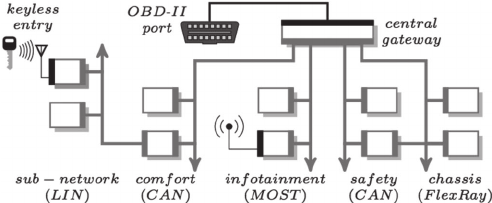
\includegraphics[width=\textwidth]{gateway.png}
	\caption{Typical Vehicle Network Infrastructure \cite{Petit}}
\end{figure}

On top of acting as an intermediate between the different sub-networks of the vehicle, the Gateway also acts as an entry point for OBD-II messages. Any message sent via the OBD-II DLC will be translated and forwarded by the Gateway to the appropriate sub-network. It comes as no surprise that this component will play a crucial role when introducing access control to the OBD-II interface.

\subsection{OBD-II}
\label{sec:obd}

\paragraph{Goal} OBD-II (On Board Diagnostics) is a specification that was introduced to allow for self diagnostic and reporting functionality for ECU's inside a vehicle, and has been mandatory in every car produced in the united states since 1996. \cite{wiki:OBD}. It allows users (testers, developers, repairmen, etc) to query ECU's about diagnostics information in order to perform a detailed analysis of the vehicles internal systems. Specifically the goals of OBD-II upon introduction were: 
\begin{itemize}
	\item Standardisation: information is communicated in a standardized format to allow for 1 tool to be used on many vehicles.
	\item Certification: Every vehicle manufacturer required to submit certification application for review and approval, which includes a detailed description of how the OBD-II protocol was implemented.
	\item Help lowering emissions by identifying emission controls in need of repair.
\end{itemize} 

The system can also be very useful in a number of other situations: A repairman looking for a specific component that is to be repaired, an employee at the factory testing all components before the vehicle is ready to be sold, a policeman analysing a vehicle after a crash to determine what caused the accident, a software developer testing the operation of a newly developed ECU, etc. 
\newline

\paragraph{Brief History} 

There were a lot of different proprietary diagnostics systems introduced over the years, before a standard arrived with the introduction of OBD-II. This brief history cited from \cite{OBDhistory} does a decent job of concisely explaining how OBD-II came to be:

\begin{displayquote}
	The origins of OBD-II actually date back to 1982 in California, when the California Air Resources Board (ARB) began developing regulations that would require all vehicles sold in that state starting in 1988 to have an onboard diagnostic system to detect emission failures. The original onboard diagnostic system (which has since become known as OBD-I) was relatively simple and only monitored the oxygen sensor, exhaust gas circulation system, fuel delivery system and engine control module.
	
	OBD-I was a step in the right direction, but lacked any requirement for standardization between different makes and models of vehicles. You still had to have different adapters to work on different vehicles, and some systems could only be accessed with costly "dealer" scan tools. So when ARB set about to develop standards for the current OBDII system, standardization was a priority: a standardized 16-pin data link connector (DLC) with specific pins assigned specific functions, standardized electronic protocols, standardized diagnostic trouble codes (DTCs), and standardized terminology.
	
	Another limitation of OBD-I was that it couldn't detect certain kinds of problems such as a dead catalytic converter or one that had been removed. Nor could it detect ignition misfires or evaporative emission problems. Furthermore, OBD-I systems would only illuminate the MIL light after a failure had occurred. It had no way of monitoring progressive deterioration of emissions-related components. So it became apparent that a more sophisticated system would be required. The California Air Resources Board eventually developed standards for the next generation OBD system, which were proposed in 1989 and became known as OBD-II. The new standards required a phase-in starting in 1994. The auto makers were given until the 1996 model year to complete the phase-in for their California vehicles.
	
	Similar standards were incorporated into the federal Clean Air Act in 1990 which also required all 49-state vehicles to be OBD-II equipped by 1996 -- with one loophole. The OBD-II systems would not have to be fully compliant until 1999. So some 1996 OBD-II systems may lack one of the features normally required to meet the OBD-II specs, such as the evaporative emissions purge test.
\end{displayquote}

\paragraph{DLC}

In order to allow a user to communicate with the vehicle's internal network, OBD-II introduces the data link connector (DLC). The DLC is a 16-pin hardware interface (although only 9 pins are specified by the standard) that is generally found close to the steering wheel (by law it is required to be installed within 0.61 m of the steering wheel) \cite{wiki:OBD}. There are 2 basic types of connectors: Type A as seen in figure \ref{fig:typeA} (using a 12V power supply) and Type B as seen in figure \ref{fig:typeB} (using a 24V power supply). the design of the two connector types prevents the insertion of a type A male plug into a type B female socket.

\begin{figure}[h]
	\label{fig:typeA}
	\centering
	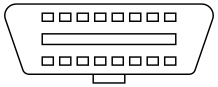
\includegraphics{typeA.png}
	\caption{Type A female connector \cite{wiki:OBD}}
\end{figure}

\begin{figure}[h]
	\label{fig:typeB}
	\centering
	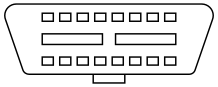
\includegraphics{typeB.png}
	\caption{Type B female connector \cite{wiki:OBD}}
\end{figure}

\paragraph{PID's}

 OBD-II introduces parameter PID's, which are codes used to identify and query specific data. The protocol is designed to work with multiple signalling protocols (the messaging protocol that is used to request and receive data from the network) but the CAN protocol is mostly implemented (Since 2008 all new vehicles sold in the us implement this signalling protocol\cite{OBDconnector}). \newline
\newline
There are multiple ways for a user to interact with this interface:
\begin{itemize}
	\item Standard Diagnostic scanning tool: a dedicated device that consists of a small hand-held module (equipped with a small screen and some buttons) connected to a male DLC-connector (The DLC inside the vehicle is always female).
	
	\item An advanced Diagnostic scanning tool that includes a DLC-connector with wifi/Bluetooth compatibility, allowing for remote diagnostics using a smartphone.
	
	\item A DLC-connector with a usb adapter allowing access via dedicated software on a pc. Since 2014 all new cars in the US support the SAE J2534 "PassThru" standard, which is a Windows API (Application Programming Interface) that provides a standard way to communicate with a car's internal buses \cite{Kosher}.\footnote{For more information on SAE J2534, see the full API reference at: https://tunertools.com/prodimages/DrewTech/Manuals/PassThru\textunderscore API-1.pdf}
	
	\item A data logger, which is designed to capture real-time data while the vehicle is in operation.
\end{itemize}

Typically the ODB-II is used like this (CAN as signalling protocol): First, the user enters the PID of the data he/she wants to query into a diagnostic tool. Second, this data is packaged in a CAN frame and sent on the CAN-bus. Third, the ECU that is responsible for the data identified by the PID in the message recognizes it as it's own, and transmits a CAN frame containing the requested data. Fourth, the diagnostic tool recognizes the response and displays the data to the user \cite{wiki:PID}. Aside from this, the OBD-II port can then be used to upgrade the ECU's firmware or to perform a myriad of diagnostic tasks.

\subsection{CAN}
\label{sec:can}


\epigraph{"Today, CAN has established itself worldwide as the backbone for the networking of embedded systems, and this not only in automotive technology"}{Dr. Siegfried Dais, Prof. Dr. Uwe Kiencke, Martin Litschel}


The CAN protocol has become a ubiquitous part of the automotive industry. In the context of internal vehicle networks, CAN messages have multiple purposes: First, there are informative messages that are designed to transmit data from and to ECU's (e.g. the Anti-Lock System (ABS) broadcasting the speed of each wheel). Second, there are action messages that are designed to request another ECU to perform an action (e.g. adaptive Cruise Control (ACC) module requesting the brakes to be applied). Third, there are the diagnostic messages defined by the OBD-II protocol. \cite{MillerB} Naturally the last type of message is the focus of this paper. The following paragraphs are dedicated to the CAN protocol.

\paragraph{Brief History} 

The history of CAN starts in 1983 when a couple of engineers at Bosch (soon aided by engineers from Mercedes-Benz and Intel) start developing a new serial bus system for use in the automobile industry. It wasn't long before CAN was officially introduced at the SAE congress in Detroit as: 'Automotive Serial Controller Area Network'. The main characteristics of this protocol were: 

\begin{itemize}
	\item An arbitration method that allows bus access to the message with the highest priority without delays.
	\item No master CAN node that is in charge of the bus.
	\item Transmitted messages are identified by their content, not by their destination or origin.
	\item This identification also determines the priority of the message within the network.
\end{itemize}

It didn't take long before the first CAN controller chips were developed in 1987 (by Intel and Philips respectively) and the first official CAN specifications were standardised in the 90's, effectively paving the way for the CAN protocol to become an industry staple as it is today. To this day Bosh has been making sure that all CAN chips comply with their proposed standards in order to avoid incompatible implementations. \footnote{For a comprehensive history of the CAN protocol confer \cite{CANhistory}}.

\paragraph{Architecture}

A typical CAN network consists of a series of nodes (with a minimal of 2 in order for the network to be functional) connected by a two-wire bus. It is important to note that there are 2 physical CAN specifications: high speed CAN (see \cite{ISO11898-2}) and low speed (or fault tolerant) CAN (see \cite{ISO11898-3}). Every CAN node consists of:
\begin{itemize}
	\item CPU: effectively the 'brain' of the node, deciding what messages are sent and taking the appropriate course of action whenever a message is received.
	\item Controller: in charge of reading and writing bits to and from the CAN bus.
	\item Transceiver: acts as in an intermediate between the bus and the controller, thereby translating between different signal levels.
\end{itemize}

This architecture specifies the minimum requirements of a CAN node. More often than not these nodes will include other components (e.g. sensors, actuators) that are connected to the CPU. It should be clear from this specification that this architecture applies to any common vehicle network (e.g. ECU's act as CAN nodes).

\paragraph{CAN Frames}

Since CAN is a message based protocol, it facilitates communication by transmitting short bursts of data called CAN frames. There are four different types of CAN frames:
\begin{itemize}
	\item Data frame: used to transmit data with a specific identifier.
	\item Remote frame: used to request the transmission of data with a specific identifier.
	\item Error frame: transmitted whenever a node detects an error on the bus.
	\item Overload frame: transmitted by a node to include a delay between data or remote frame.
\end{itemize}

There are 2 frame formats: base frame format and the extended frame format. The only difference being that the extended frame format uses a 29 identifier bits and the base frame format only uses 11. Table \ref{table:1} lists all the fields of a base format data frame. The extended frame format is the same except for an additional identifier field (18 bits) right after the identifier extension bit (IDE) field.

\begin{table}[]
	\begin{tabular}{|l|l|l|}
		\hline
		\rowcolor[HTML]{9B9B9B} 
		name & size (bits) & purpose \\ \hline
		start-of-frame & 1 & Denote start of transmission \\ \hline
		identifier (ID) & 11 & Unique identifier + determines priority \\ \hline
		remote transmission request (RTR) & 1 & must be 1 for remote frames \\ \hline
		identifier extension bit (IDE) & 1 & must be 1 for extended frames \\ \hline
		reserved bit & 1 & reserved for future use \\ \hline
		data length code (DLC) & 4 & length of data field \\ \hline
		data field & 64 & data to be transmitted \\ \hline
		cyclic redundancy check (CLC) & 15 & check for errors \footnotemark  \\ \hline
		CRC delimiter & 1 &  must be 1 \\ \hline
		acknowledgement slot (ACK) & 1 & used for message acknowledgement \\ \hline
		ACK delimiter & 1 & must be 1 \\ \hline
		end-of-frame (EOF) & 7 & must be 1  \\ \hline
	\end{tabular}
\caption{base frame format \cite{wiki:CAN}}
\label{table:1}
\end{table}

\footnotetext{A cyclic redundancy check is a way of detecting accidental changes to transmitted data (e.g. due to noise, interference, etc). For more information on cyclic redundancy checking see \cite{wiki:CRC}.}

\paragraph{Data Transmission}

The operation of the CAN protocol is pretty straightforward: a node transmits a message with a specific ID on the bus. Any node that is connected to the same bus is able to receive the message (broadcast), but only the nodes that are listening for this specific ID will take action. It is worth noting that the ID is used to identify the content, not the sender or receiver. As a matter of fact CAN does not provide any way of authenticating the sender or receiver, which results in various security related difficulties (see \ref{sec:issues}) . Aside from identifying the content, this ID is also used to solve the issue of message arbitration. CAN is a carrier sense multiple access protocol, whereby each nodes observes the bus before transmitting data on it, if it detects that the bus is in use it waits for some time before trying again. This does not prevent nodes from starting a data transfer at the same time, this is where bit wise message arbitration provides a solution. \cite{CANarbitration}.

\paragraph{Bit wise message arbitration}

Whenever 2 (or more) nodes initiate a transmission on the bus at the same time, bit wise message arbitration is performed. Every bit of the message ID can be either 1 or 0. The CAN specifications use the term dominant (logical 0) and recessive (logical 1). These terms originate from the fact that whenever more than one bit is simultaneously written to the bus, and one of these is dominant, the dominant bit 'wins', meaning a logical 0 will be seen on the bus. Whenever a node transmits a logical 1 but sees a logical 0, it realizes that there is a contention and re-queues its message for later transmission. Since the identifier is transmitted at the start of the CAN frame, the node with the numerically lowest identifier transmits more zeros at the start of the frame, and that is the node that wins the arbitration. Concisely put we can say that messages with lower ID's have priority over messages with higher ID's. The decision to identify messages by their content (instead of their sender or receiver) is motivated by the fact that certain very important types of messages (e.g. errors) can be given a very low id, thereby ensuring they are less prone to be delayed. This approach does introduce some issues when it comes to security (see \ref{sec:issues}).

\paragraph{Layering}

In line with most networking protocols, it is common practice to decompose them into different abstract layers. This is done to simplify the design and make modularisation easier \cite{wiki:ProtocolStack}. In the case of CAN the layers are:

\begin{itemize}
	\item \textbf{Application layer:} OBD-II, CANOpen, VulCAN etc.
	\item \textbf{Object layer:} message filtering and status handling.
	\item \textbf{Transfer layer:} error detection, message arbitration, bit timing, etc.
	\item \textbf{Physical layer:} signal voltages, pin-out configuration, etc.
\end{itemize}

For more information on the CAN protocol see \cite{ISO11898-2} and \cite{ISO11898-3}.

\subsection{OBD-II Security Issues}
\label{sec:issues}

\epigraph{"CAN, by design, offers no protection from manipulation"}{Dan Klinedinst, \\ Christopher King}

It is a well-known fact that the automotive industry has always considered safety a critical engineering concern (especially since the public awareness around lethal accidents has only increased over the years). Unfortunately it is unclear whether developers (especially concerning the internal network) have considered the security in their design. However it seems this is not the case because of three reasons. First, there is no inherent support for addressing, encryption or authentication \cite{MillerB}. Second, most of the networks and ECU's were designed when access to the bus required physical access to the vehicle, therefore security was not a primary concern. Third, speed and timing are deemed more important to the safety and performance of the vehicle than data security \cite{Klinedinst05}. This vulnerability is worsened by the fact that the attack surface for modern automobiles is growing swiftly as more sophisticated services and communications features are incorporated into vehicles \cite{Kosher}. The OBD-II specification is one of these since the interface it introduces provides direct access to the internal vehicle network. This allows malicious agents to easily construct and insert CAN messages to alter the vehicle's behaviour, as has been frequently demonstrated by Charlie Miller and Chris Valasek's exploits \cite{MillerA}\cite{MillerB}\cite{MillerC}. Before analysing the attack vectors that OBD-II introduces, and the possible impact thereof on the safety and security of the vehicle, let's first take a closer look at CAN's shortcomings when it comes to safety.

\subsection{CAN security challenges}
\label{sec:can_challenges}
The CAN protocol has a number of inherent vulnerabilities that are common to any implementation. The most obvious and important ones are:

\begin{itemize}
	\item \textbf{Broadcast nature:} CAN frames are both physically and logically (no destination address) broadcasted on the network. This means that a malicious node on the bus can snoop on all communications or even worse: send packets to any other node on the network \cite{Kosher}. 
	
	\item \textbf{No authentication:} CAN frames do not have source identifier fields, so there is no way for any node to be aware of the source of any messages it receives. This means that any compromised component (or any other form of unsanctioned access to the CAN bus for that matter) can inject arbitrary messages. Whereas the system has no way of knowing these messages were not sent by the appropriate component \cite{Kosher}\cite{CANissues}.
	
	\item \textbf{No encryption:} We've mentioned that speed and timing are deemed more important to the safety and performance of the vehicle than data security. A clear result of this is the decision to omit any encryption capabilities. This is because the limited  computational power of ECU's makes it difficult to implement robust cryptographic algorithms. \cite{CANissues}.  
	
	\item \textbf{Susceptibility to Denial of Service (DoS):} This problem arises mainly from the protocol's message arbitration method. Any malicious node can effectively spam the bus with high priority messages (only zeroes as ID) causing all other nodes to back off (no protection against "babbling idiots"\cite{Pike15})\cite{Kosher}.
	
	\item \textbf{Not Byzantine fault tolerant:} In most distributed systems, malicious attacks and software errors can cause a node to exhibit Byzantine (i.e. arbitrary) behaviour\cite{Byzantine}. Because of the distributed nature of any CAN system, there is imperfect information on whether a component has failed (or has been compromised by attack) or not. This could result in situations where entire system services fail since a common consensus cannot be reached\cite{wiki:ByzantineFault}. \footnote{For more information on Byzantine faults, and how it is tolerated in a system see \cite{Byzantine} and \cite{wiki:ByzantineFault}.}.
	
\end{itemize}

\subsection{OBD-II security challenges}
\label{sec:obd_challenges}

 From the discussion on CAN's security vulnerabilities it is clear that any CAN implementation, and by extension the application layer protocols that run on top of it, are not secure by default. OBD-II is certainly no exception. The OBD-II port can access all CAN buses that make up the vehicle network. This is vital since service technicians should be able to diagnose and update almost any ECU in a vehicle\cite{Kosher}. The high level of access technicians have over the vehicle they are diagnosing/repairing is not privileged however. Anyone with physical access to the vehicle, and in possession of the right tools, is granted the same level of access. The problem here is that the system has no way of knowing which OBD-II connections are to be trusted and which aren't, which is exactly the problem this paper attempts to address. Before looking at some example OBD-II exploits, it is a good idea to define a sufficient attacker model first.

\subsection{Attacker model} 
\label{sec:attacker_model}
Here, an attempt is made to define the types of attackers that this paper aims to defend against. a similar classification as \cite{Maxim} and \cite{Petit} is followed:

\begin{itemize}
	\item \textbf{Insider or outsider:} The insider is considered an interactive member of the network, meaning he/she can communicate with other members freely. The outsider however is limited in the diversity of attacks he/she can mount.
	
	Classification: \textbf{outsider}, since the attacker is not part of the CAN bus. It is worth noting however that when the attacker uses the OBD port to mount an attack, he/she can communicate with the other nodes on the bus. This however is treated by this paper as part of a successful attack, not as an a priori capability of the attacker.
	
	\item \textbf{Malicious or rational:}  A malicious attacker exploits the system for reasons other than personal gain, making them more unpredictable since their motives and resources can vary. A rational attacker however is motivated solely by personal profit, be it money or fame, making them more predictable.
	
	Classification: \textbf{both}, since an attacker using the OBD port as attack vector could be both malicious (e.g. Endangering the life of a rival) and rational (e.g. lowering the internal odometer value before selling the vehicle).
	
	\item \textbf{Active or passive:} An active attacker is able to generate and transmit messages, whereas a passive attacker is constrained to eavesdropping.
	
	Classification: \textbf{active}, since we know the attacker can have access to tools (e.g. PassThru) that grant him/her active capabilities.
	
	\item \textbf{Local or extended:} This criterion is based on the scope of the attacker. A local attacker has only limited attack vectors, whereas an extended attacker has access to lots.
	
	Classification: \textbf{local}, since a comprehensive analysis of multiple attack vectors, although touched upon in section \ref{sec:other_attack_vectors}, is considered out of scope for this paper (c.f. \cite{Pike15}\cite{Kleberger15}\cite{Russel17}\cite{MillerA}\cite{Petit}\cite{Kosher}\cite{Kosher2}\cite{Bayer15}).
\end{itemize}

\subsection{Example attacks}
\label{sec:example_attacks}
 Let us take look at some examples of attacks that adhere to the model proposed earlier. The exploits that are presented here were performed by Charlie Miller and Chris Valasek, in an effort to raise awareness about the issue, as well as allowing car manufacturers to build safer cars in the future. They accomplished this by not only finding and exploiting various vulnerabilities in extant vehicles, but also sharing any software that made these exploits possible. An example of this is EcomCat, which is software written in C to aid in the reading and writing of data to the CAN bus through one or more Ecom cables \cite{MillerC}. Figure \ref{fig:exploitsetup} shows the physical setup of the exploits, whereby a laptop is connected to a car's OBD-II port via an Ecom cable, allowing the researchers to use their EcomCat software to inject their own CAN messages onto the internal bus. Although seemingly straightforward there are many potential problems in attempting to make the vehicle perform actions by injecting packets on the CAN bus. First, not everything can be controlled via the CAN bus (e.g. cruise control). Second, if a specific type of CAN packet is found to be a request (An ECU asking for another ECU to perform an action) replaying a fake copy does not guarantee that the message is accepted. This is because the original message is still sent, possibly confusing the ECU with conflicting information. Third, It is also possible that fake messages are ignored because of built-in security features inside the ECU. Despite these difficulties these researchers did manage to mount a series of interesting exploits, two of which are presented here.

\begin{figure}[h]
	\label{fig:exploitsetup}
	\centering
	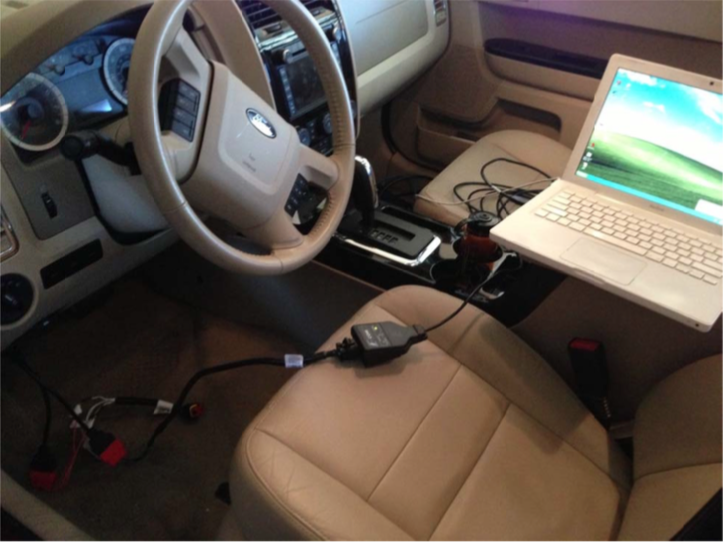
\includegraphics[width=\textwidth]{ExploitSetup.png}
	\caption{The setup of the exploit \cite{MillerC}.}
\end{figure}

\paragraph{Speedometer} In this example ,performed on a 2010 Toyota Prius, the researchers managed to identify the messages that are sent to the speedometer to display the current velocity of the vehicle. Replaying this message with custom data fields allowed them to display any arbitrary speed on the speedometer display, as can be seen in figure \ref{fig:speedometer}.

\begin{figure}[h]
	\label{fig:speedometer}
	\centering
	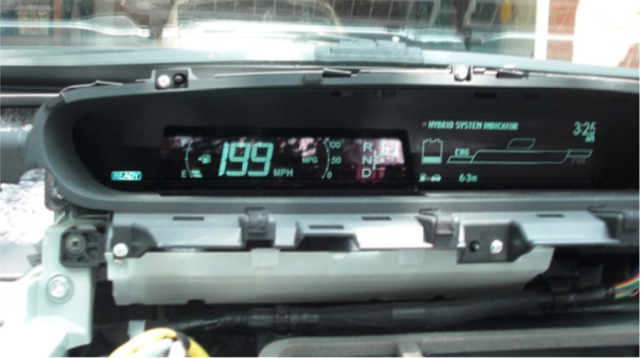
\includegraphics[width=\textwidth]{speedometer.png}
	\caption{Speedometer showing an arbitrary value \cite{MillerC}.}
\end{figure}

\paragraph{Denial of Service} Here the researches cleverly take advantage of how the CAN protocol works. Remember from \ref{sec:can} that CAN uses priority scheduling over the ID's of the messages that are sent on the bus. This means that spamming a high priority message would prevent all other messages from being transmitted. This vulnerability is exploited here by flooding the bus with CAN messages with an ID of 0. In figure \ref{fig:DoS} we can see the result of this attack when the engine is turned off. This flooding of the CAN bus halts the engine from being turned on, as well as putting the system in an all out state of disarray (as can bee seen from the various warning symbols on the instrument cluster).
 
\begin{figure}[h]
	\label{fig:DoS}
	\centering
	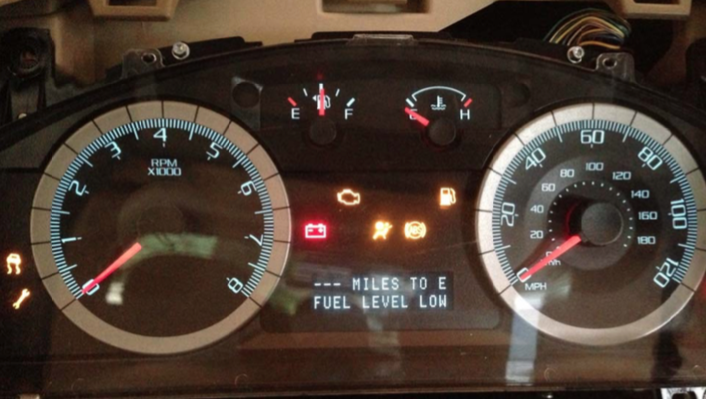
\includegraphics[width=\textwidth]{DoS.png}
	\caption{Denial of service of a vehicle CAN bus \cite{MillerC}.}
\end{figure}

\paragraph{Diagnostic session} The aforementioned examples used injection of messages that are normally sent from ECU to ECU, thereby erroneously invoking actions from certain ECU's. Another approach is to trick the vehicle network into starting a diagnostic session. These are used in normal circumstances by a technician at a garage. It allows them to test the function of an ECU without having to take the vehicle on the road, as well as recalibrating them. Starting a diagnostic session does require circumventing an authentication procedure (see \ref{sec:obd_access_control}) but this proved rather easy (they did this by reverse engineering an official authentication device and extracting the keys). Once a diagnostic session was established it opened up a wide array of possible attacks: Killing the engine, disabling the brakes, honking the horn, unlocking/locking doors, and even reprogramming of certain ECU's (see \cite{MillerC} for a detailed description of the attacks).

\paragraph{Impact} It is clear that the level of control that is obtainable via the OBD-II port is worrying. Especially if we consider that there exist OBD-II devices with Bluetooth or Wifi capabilities, allowing attacks to be mounted from a distance (imagine a DoS attack being mounted while driving a car at high speed). It is these scenarios that elevate the concern from mere vehicular integrity, to concern over the physical safety of the driver and his/her passengers. Sure it could be stated that this danger originates from a malicious agent gaining illegal access to the vehicle, rather than the security of the internal vehicle system. But this conclusion would gloss over the fact that the OBD-II interface was designed to be used only by repairman, testers, policemen, etc. Therefore it is only logical that this privileged use is enforced by the system, rather than being merely implied.

\section{Related work}
\label{sec:related_work}

\paragraph{Introduction} Before moving on to our proposed solution let's take a look at some papers that are relevant to this subject. A lot of these, while not really tackling the same problem as proposed here, were a vital influence on this paper. A closer look at the contributions they provided is definitely in order. First, we discuss a paper that attempts to meet one of the challenges of this paper, namely by introducing access control to the OBD-II interface. Second, some of the possible attack vectors that haven't been discussed so far are introduced, as well as the papers that surveyed them. Third, a summary is made of different proposed application layer CAN protocols that were designed to remedy CAN's inherent security issues. Fourth, another summary of security solutions is presented, but this time regarding external instead of internal vehicle security. Last, we mention some proposed security frameworks and assurance levels that were proposed for the automobile industry.

\subsection{OBD-II Access Control}
\label{sec:obd_access_control}

The paper discussed here (see \cite{Yadav16}) is relevant since it, like this paper does, states that the OBD-II interface in modern cars exposes the internal system to a myriad of different attacks (see \ref{sec:example_attacks} for some examples). On top of sharing this insight, the paper also proposes to improve on a solution that was deemed insufficiently secure (the seed key algorithm), as well as implementing them in a small demo. These solutions will be discussed next.


\paragraph{Seed key algorithm} The seed key algorithm (like the name implies) applies a secret key value to calculate the response key from a randomly generated seed. Only the person with the correct secret key can gain access to the diagnostic service of a specific ECU. The idea is that a dedicated and trusted device would be distributed, this device would contain the secret key, and allow authenticated diagnostic sessions with the ECU's inside the vehicle. This solution was stipulated by another paper (see \cite{Bayer}) and has already been implemented in a lot of vehicles (see \ref{sec:example_attacks}, diagnostic session). The problem with this algorithm is the fact the same ECU in different cars will have the same secret key. Another problem is that the secret key material is often stored in unprotected memory. If enough keys are made public this would undermine the security of the entire algorithm.  

\paragraph{Two-Way authentication method}
This algorithm is an extension of the seed-key algorithm. In addition to requiring possession of the secret key, a message will be sent to the client of the vehicle whenever access is requested (Cellular or via Internet). Without acknowledgement from the user the seed is dropped and access is denied. The above process adds a layer of safety as a result of keeping the client informed at every stage.

\paragraph{Timer Method}  
The timer method is again an extension of the Two-Way authentication method. It Exploits the time brute force methods and other algorithms take to crack a 16-bit long seed key, as well as giving more autonomy the car owner by giving the global seed directly to the client, who in turn must enter the key to complete the authentication process. As soon as a security access request is sent by the tester, the timer will be started. As soon as the timer runs out, a message or a notification alert is sent to the client informing about the malicious activity, as well as aborting the authentication process. 

\paragraph{Discussion} 
The two extensions offered by this paper do not actually help prevent most of the original algorithms shortcomings. The key oversight that is made here is that the added security comes from a dedicated device that is tasked with performing the additional authentication procedures (e.g. sending a message for the two-way authentication method and starting a timer for the timer method). There is nothing preventing anyone from circumventing these by using anything other than this dedicated device to gain access to the system (e.g. computer connected directly to the OBD-II port). 

\subsection{Other attack vectors}
\label{sec:other_attack_vectors}

A couple of possible attack vectors have been discussed already (OBD-II in section \ref{sec:obd_access_control}, Bluetooth in the context paragraph of section \ref{sec:introduction}). Let's take the time to look at some other attack vectors that were proposed. We will follow the same general classification of these attack vectors as in \cite{Kosher}: indirect physical access (those that require physical access to the vehicle or via an intermediate), short-range wireless and long range wireless.\footnote{It should be clear that the OBD-II interface belongs to the indirect physical access class of attack vectors, while Bluetooth is considered a short-range wireless kind of access.}

\subsubsection{Indirect physical access}

\paragraph{Entertainment: Disk, USB and IPod} It is hard to find any new vehicle that does not include the ability to play an audio cd, plug in a usb audio device, or directly connect with an Apple IPod or Iphone in order to play music. It is not unthinkable for a someone to encode malicious input onto a CD, and distributing them to non-suspecting targets. To go from a CD or USB drive to an audio stream, the input must interact with many hundreds of thousands of lines of code throughout a stack of software components, which could contain vulnerabilities that could be exploited to take control of the system\cite{Pike15}. Corrupting a vehicle's CD-player might be considered a fairly innocent attack, but these are often connected with other, more safety-crucial systems. This is the reason why entertainment systems should be seriously considered when potential attack vectors are surveyed.

\subsubsection{Short-range wireless access}

\paragraph{Remote Keyless Entry} Today, almost all automobiles shipped in the U.S. use RF-based remote keyless entry (RKE) systems to remotely open doors, activate alarms, flash lights and, in some cases, even start the ignition\cite{Kosher}. In these systems the radio transmitter sends encrypted data containing identifying information from which the ECU can determine if the key is valid\cite{MillerA}. mounting attacks with regards to remote code execution in this way is infeasible. However it has been shown that in some cases it is possible to unlock/start the car without the proper key fob (see \cite{KeeLoq}), which would result in unauthorised access being granted.

\paragraph{RFID car keys} A Radio-frequency identifier (RFID) immobilizer, also called passive anti-theft system (PATS), is a chip embedded in the top part of an ignition key. This chip sends out an encrypted string of radio-frequency signals when the driver inserts it into the ignition-key slot. Without this code, the car either won't start or won't activate the fuel pump. So even if someone hotwires the car or copies an ignition key, the car is not going to start because it hasn't received the proper radio-frequency code\cite{RFID}. As with RKE, this does not provide a significant attack surface.\cite{MillerA}

\paragraph{TPMS} The tire pressure monitoring system (TPMS) are designed to alert drivers about under or over inflated tires. The most common form of such systems uses rotating sensors constantly measuring the tire pressure and transmitting real time data to an ECU (frequently in similar bands as RKEs)\cite{Kosher}. While the attack surface is also small here, It is has been shown that it is possible to perform some actions against the TPMS, such as causing the vehicle to think it is having a tire problem\cite{TPMS} or in some cases even crashing the ECU that the data is sent to\cite{MillerA}. Alternatively TPMS could be used to track the car from a distance\cite{TPMS}. These problems could be solved by introducing some detection mechanism to raise an alarm when detecting frequent conflicting information, as well as encrypting and authenticating the TPM packets sent by the sensors\cite{TPMS}.

\paragraph{V2V, V2I and V2N} While the technology is fairly new, a lot have car manufacturers have started to introduce more external connectability to the vehicles they produce. This can take on many forms\cite{Ahmed}. First, vehicle-to-vehicle (V2V) connections are mainly introduced in the context of self driving cars who communicate with each other to avoid collisions (see \cite{Enisa}). Second, there are vehicle-to-infrastructure connections. Think of a car automatically paying for gas without the need for the driver to do so. Or a repair shop diagnosing a car from a distance (see \cite{Kleberger}). Third, there's vehicle-to-network communication. There is a considerable amount of literature that attempts to address the concern around this newly emerging technology, for more information on the subject we refer the reader to these (see \cite{Kleberger15}\cite{Russel17}\cite{Maxim}\cite{Crispo}.

\subsubsection{Long-range wireless access}

A distinction can be made between two types of long-range wireless access methods. First, there are addressable channels, which are specifically directed towards an automobile. Second, there are broadcast channels, where typically an automobile "tunes in" on demand. A prime example of the latter is GPS.

\paragraph{GPS} Global positioning systems (GPS) are used in automobiles to accurately determine it's position as well as guiding them to user specified locations. GPS does not provide a significant remote attack surface, since GPS signals are predominantly processed by custom hardware\cite{Kosher}. However some attacks have been successfully proposed. First, there's GPS jamming where cheap device (approximately 20 dollars) is used to jam all GPS signals in the area. This could be used by a car thief to prevent a car's anti theft system of knowing where the vehicle is. \footnote{In these types  of systems a message is sent to the owner of the car whenever a location change is detected by the GPS system and the owner is not present in the vehicle.} Second, There's GPS spoofing, where normal GPS signals are replicated, providing false locations. These could again be used to counter location based anti theft systems \cite{Petit}. Multiple mitigation techniques are presented in \cite{GPS1} and back-office countermeasures to counter GPS jamming and spoofing are presented in \cite{GPS2} and \cite{GPS3}. 

\paragraph{Radio} Another broadcast channel is radio signals, these can either be standard AM/FM radio (Digital Radio) or satellite radio. These signals are simply converted to audio output upon reception, so they are not likely to contain exploitable vulnerabilities. However, the Radio Data System data that is used to send information along with FM analogue signals (or the equivalent on satellite radio) can be a vulnerability. Since the radio unit is often connected to the in-vehicle network and because radio data needs to be parsed and displayed (think of artist and songtitle data). These vulnerability could be fixed by ridding the radio data code of any bugs that could be exploited, as well as introducing input validation and sanitation on any data that is received\footnote{Input validation consists of checking if the received information meets a particular set of criteria. Input sanitation on the other hand consist of modifying this information to ensure it meets these criteria}. \cite{MillerA}\cite{MillerD}\cite{Kosher}. 

\paragraph{Vehicle Telematics} Vehicle telematics is a broad term, that encompasses nearly all addressable communication channels of a vehicle. They typically use cellular voice and data systems to provide continuous communication with the vehicle (e.g. General Motor's OnStar system, Toyota's SafetyConnect, Lexus' Enform, BMW's BMW Assist, and Mercedes-Benz' mbrace). These systems provide a broad range of features like crash reporting, diagnostics (reporting a mechanical issue to the owner) and anti-theft (location based anti theft systems)\cite{Kosher}. Due to it's characteristics (long distance, high bandwidth, addressable, etc) these systems are considered the holy grail of automotive attacks\cite{MillerA}. In 2015 an article was published in Wired magazine (see \cite{Wired}) documenting the work of 2 researchers (Charlie Miller and Chris Valasek) and their attempt at remotely hacking into a 2014 Jeep Cherokee exploiting it's telematics system (UConnect). They were able to remotely disable the brakes, honk the horn, jerk the seatbelt and even take control of the steering wheel\cite{Wired}. The number of vehicles that were vulnerable were in the hundreds of thousands and it forced a 1.4 million vehicle recall by Fiat-Chrysler (who also own the Jeep automotive brand).\footnote{for more information on this famous exploit see \cite{MillerD}.}

\subsubsection{Future Systems}
What should be considered is that the automotive industry is rapidly evolving. what is considered a critical safety concern today might be nullified by a new innovation. But more importantly these new innovations might come with their own safety critical concerns. One example of this is discussed here (Intelligent transportation systems), however it should come as no surprise that there are many other future designs that will have to be researched.

\paragraph{ITS} Intelligent transportation systems (ITS) or in this case more commonly referred to as self-driving cars are automated vehicles that require barely any user interaction while moving. they are based on communication of data among vehicles (V2V) and/or between vehicles and the infrastructure (V2I/I2V) to provide this new functionality. Although innovative and potentially a solution to a couple of serious transportation-related issues (e.g. congestion, accidents, etc) it has been shown in \cite{Petit} that this also introduces a couple of interesting new attack vectors:   

\begin{itemize}
	\item \textbf{infrastructure signs:} Any decent ITS should be able to recognise and interpret road signs in order for them to adhere to local traffic regulations. However, can these systems make the distinction between an official road sign, and a fake one made by a malicious agent in an attempt to cause mayhem.\cite{Petit}
	
	\item \textbf{Video Image Processing} Besides detecting and interpreting road signs the ITS should be able to correctly interpret it's surroundings (e.g. width of the road, speed bumps, other vehicles, pedestrians, etc). This technology will probably be provided by artificial intelligence (AI) systems (also called machine vision) that are trained to detect certain objects. Any vulnerabilities found in these systems could be exploited, again causing significant chaos (e.g. painting an image on the road that tricks automated vehicles into thinking someone's crossing the road).\cite{Petit}
	
	\item \textbf{GPS} It should be obvious that any ITS will rely heavily on GPS to automatically navigate. A GPS jamming/spoofing device in the wrong hands would be a powerful tool allowing them to influence the navigation of all automated vehicles within the action radius of the device.\cite{Petit}
	
	\item \textbf{Acoustic Sensors} These could be used by an ITS to detect a known signal (e.g. a car crashing). Again it opens up the possibility for attackers to look for vulnerabilities in how these signals are processed. This would allow them to falsely trigger events (e.g. playing a modulated crashing sound on a stereo causing the airbag to be triggered and brakes to be angaged), as well as using jammers to block the sensors from correctly interpreting any sounds.\cite{Petit}
	
	\item \textbf{Radar and Lidar} Because of the shortcomings of video image processing discussed earlier, it should be possible for the vehicle to detect physical objects. Radar and Lidar (Using light instead of sound to detect objects) could be used here. Again jamming/spoofing devices could be developed that interfere with the detection systems.\cite{Petit}
\end{itemize}

\subsection{Internal Vehicle Security}

In the previous section (see \ref{sec:other_attack_vectors}) the most important attack vectors of modern automobiles are discussed. Defending against these requires a specific measure per vector, meaning no solution will confidently prevent attacks over all surfaces. Take TPMS for example, the solution here is to define a way of communicating between the tire pressure sensors and the TPMS ECU that cannot be spoofed or interfered with. This approach is fine but it doesn't address a greater issue with in-vehicle networks. Namely, once access to the network is attained, an attacker is unbounded in which ECU's it can communicate with and what messages it sends to them (if no additional security measures are implemented of course). This vulnerability is an inherent flaw of the network communications protocol (CAN in our case). In section \ref{sec:can} (Layering) the layered nature of the CAN protocol was discussed. What if an application layer extension of the protocol was introduced that alleviates the aforementioned security issues? This would mean that even is access is attained, this breach will be confined to the ECU that was used as an attack vector, severely limiting the scope of the attack. Fortunately these solutions have been proposed and a selection of them will be discussed next.

\subsubsection{VulCAN} 
VulCAN is a generic design for vehicular message authentication, software component attestation and isolation. This solution is distinguished from previous work (e.g. CANcrypt\cite{Pfeiffer}, VatiCAN\cite{VatiCAN} and Leia\cite{Leia}) by relying on trusted hardware and a minimal trusted computing Base (TCB). This TCB relies heavily on the SANCUS\cite{Sancus} security architecture. the goal of SANCUS is to provide network embedded systems with remote attestation and strong integrity and authenticity guarantees with a minimal hardware TCB. Figure \ref{fig:SANCUS} shows the SANCUS system model. The infrastructure provider (IP) provides a number of nodes (Ni) on which software providers (SPi) can deploy software modules SMj,k. This model is applicable to many ICT systems today (in the case of VulCAN this system of course a CAN network).\cite{Sancus} VulCAN uses SANCUS to compartmentalise every ECU into a small group of trustworthy authenticated software components. It does so by introducing the following security features: 

\begin{itemize}
	\item \textbf{Message Authentication}: The system uses MAC's (message authentication codes) to prove the message was indeed sent by a trusted sender component.\cite{VulCAN}
	
	\item \textbf{Lightweight Cryptography}: Lightweight cryptography is a must because of strict timing constraints and because of the computational limitations of the embedded devices.\cite{VulCAN}
	
	\item \textbf{Replay Attack Resistance}: the authentication scheme is immune to replay attacks (a malicious agent injecting a previously sent message in the hope of it being falsely authenticated). This is ensured by using short term session keys, and a monotonically increasing counter or nonce as a source of freshness in the MAC computation.\cite{VulCAN}
	
	\item \textbf{Backwards Compatibility}: Legacy unmodified applications without authenticated communication should continue to function. To this end the system broadcasts the authenticated message in plain text, and afterwards constructs and transmits authentication data on a different CAN identifier, effectively decoupling the authentication metadata from the original message.\cite{VulCAN}
\end{itemize}

\subsubsection{CANCrypt} CANcrypt uses a CAN feature that allows two devices to exchange a hidden bit that is not visible to other CAN devices. This allows generating pairing keys that only the two devices know. CANcrypt uses a dynamic 64-bit key to cover the longest possible secure data block, 8 bytes. From this key, a pseudo one-time pad is generated and changes frequently. CANcrypt does not protect against DOS attacks.\cite{Pfeiffer}.

\begin{figure}[h]
	\label{fig:SANCUS}
	\centering
	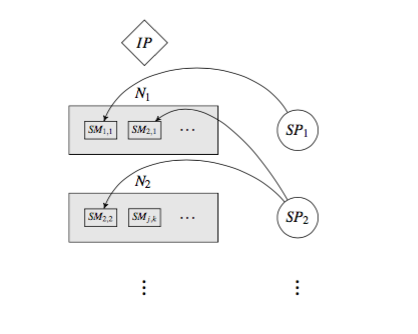
\includegraphics[width=\textwidth]{SANCUS.png}
	\caption{SANCUS \cite{MillerC}.}
\end{figure} 

\subsubsection{VatiCAN} VatiCAN is a framework for embedded controllers connected to the CAN bus, which allows both senders and receivers to authenticate exchanged data. It introduces some the same features that VulCAN does: MAC's for message authentication, nonces to prevent replay attacks and backward compatibility. However, it also introduces a new feature, namely spoof detection and prevention. spoofed messages are detected by monitoring messages with its own sender identification (remember that CAN messages are broadcasted over the entire network). If a component detects a message with its own sender ID, it must be a spoofed message. Once spoofing is detected it can still be prevented (the ID is the first thing that is sent over the bus). This is done by writing dominant bits (zeros) to the bus, effectively invalidating the CRC bits while the spoofed CAN frame is still being processed.\cite{VatiCAN}

\section{Preliminaries}
\label{sec:preliminaries}

This section serves as a technical primer to all the security related software solutions that are employed in this paper. An in-depth discussion of these topics is considered out of scope. First, the main characteristics of microcontrollers are presented. Second, the concept of role-based access control is introduced. Third, the reader is familiarised with public key cryptography, and what sets it apart from symmetric cryptography. Fourth, we will take a look at how secret keys (asymmetric or symmetric) are established between two parties. Fifth, we will explain how public key cryptography can be used in the context of authentication. Sixth, the concept of hashing and why it i useful is explained. Seventh, the concept of security level is concisely explained. The last chapter of this section gives an overview of all the specific implementations that were selected by the researchers of this paper, as well as motivating these decisions. The reader should keep in mind that the selection of algorithms and systems selected here is far from comprehensive, only those that are relevant to the solution presented in this paper (see section \ref{sec:solution}) are discussed. 


\subsection{ECU Microcontrollers}
As discussed before, an ECU is an embedded computer that is designed to perform a specific function. The core of any ECU is a small computer on an integrated circuit called a microcontroller. A microcontroller consists of one or more central processing units (CPUs)  along with memory and programmable input/output peripherals. There a couple of characteristics of microcontrollers that are touched upon in the course of this paper, so a description of these characteristics is given next:

\begin{itemize}
	\item \textbf{Word size:} The word size of a microcontroller (or any computer for that matter) is the natural unit of data used by a particular processor. A word is a fixed-sized piece of data handled as a single unit by the instruction set or the hardware of the processor. The number of bits in a word, called the word size, is an important characteristic of any microcontroller. Within the context of ECU's, word sizes of 8 bits (e.g. driver information), 16 bits (e.g. vehicle control) and 32 bits (power train) are most common.\cite{ECU}
	
	\item \textbf{Clock rate:} The clock rate of a CPU refers to the rate at which it processes words of data. it is used as an indicator of the processor's speed. It is measured in clock cycles per second or hertz (Hz). 
	
	\item \textbf{Memory:} There are two basic types of memory: data memory and program memory.
	\begin{itemize}
		\item \textbf{Data Memory}: Data memory is where variables and all intermediate calculations are stored by the CPU. It is generally implemented by RAM \footnote{random access memory (RAM) is a type of memory where individual data can be read or written in almost the same amount of time irrespective of the physical location of data inside the memory.}. This data is often volatile, meaning the data is lost when power is removed.
		
		\item \textbf{Program memory}: Program memory is where the application is stored, i.e. the code itself. This type of memory is implemented using non-volatile storage technologies like ROM \footnote{Read-only memory (ROM) is a type of non-volatile memory where the data stored can not be modified (or where it is considered very difficult to do so).}, EPROM\footnote{erasable programmable read-only memory (EPROM) is a non-volatile type of memory that can be erased (by exposing the chip the ultraviolet light) and reprogrammed.}, EEPROM\footnote{Electrically erasable programmable read-only Memory (EEPROM) is a type of non-volatile memory that can be erased and reprogrammed electronically.} or Flash Memory\footnote{Flash memory is type of EEPROM  that can be electrically erased and reprogrammed much faster than regular EEPROM chips by using large erase blocks.}.
	\end{itemize}
	
	\item \textbf{Serial Communications Interfaces:} Serial communications is a way of communication in computer networks where bits are transmitted one bit at a time (e.g. CAN). This is in contrast to parallel communications where a link is used with several parallel channels, allowing multiple bits to be sent at the same time (e.g. USB). Most microcontrollers offer dedicated hardware allowing for easy communication with other devices (e.g. CAN controller).
	
	\item \textbf{Others:} Most microcontrollers offer various other hardware like: a timer, an analog-to-digital convertor (ADC) that allows for an analog signal (like the output of a sensor) to be transformed into a digital signal, a clock generator, etc.
\end{itemize}

\subsection{Role-Base Access Control}
\label{sec:RBAC}

Role-based access control (RBAC) is a well-defined way of restricting system access to authorized users. It especially useful in large enterprises where roles are created for various job functions. Each role is assigned the necessary permissions to interact with a secured system (e.g. the company database, the local private network, development software, etc). The idea is that a worker is assigned a role based on what he/she requires to do his/her job, and nothing more. This way it is avoided that workers are granted permissions they do not require. There are two basic types of RBAC\cite{wiki:RBAC}:

\begin{itemize}
	\item \textbf{Mandatory Access Control:} In a system where mandatory access control (MAC) is a enforced, only the administrator of the system is able to create and assign roles. This is done by defining a security policy that users are unable to override or alter. The administrator of the system is called the security policy administrator.
	
	\item \textbf{Discretionary Access Control:} When discretionary access control (DAC) is enforced, it is up to the users themselves to make policy decisions and/or assign security attributes.
\end{itemize}


\subsection{Public Key Cryptography}
\label{sec:PKC}

\paragraph{Cryptography} The primary goal of cryptography in general is to allow for secure communication between two parties. This means that protocols are designed that prevent third parties or the public in general from reading private messages. This is done by encrypting the message, which consists of converting the information from a readable state to apparent nonsense. Only the intended recipient should be able to restore the information to it's original form, which is called decryption. To allow for this to work, the procedure of encryption and decryption should only be possible by the sender and the receiver respectively. Generally this procedure consists of two parts. First, there is the cypher, which is the algorithm that does the actual conversion. Second, there's the secret key, which is used by the cipher together with the input (plaintext) to create the encrypted output (ciphertext). The main advantage of this architecture is that the chosen cipher can be made public, as long as the key is kept secret. The receiver of the secret message, who is in possession of the same secret key, runs the same cipher in reverse with the secret key and the ciphertext as inputs, yielding the original plaintext.\cite{wiki:Cryptography}

\paragraph{Symmetric vs Asymmetric}The procedure outlined above is called symmetric key cryptography since both parties are in possession of the same secret key. The disadvantage here is that these keys need to be securely exchanged beforehand (e.g. via a secure channel) to allow for secure communications. Asymmetric (or public key) cryptography offers a solution to this problem. In this case a key pair is created where each one serves a specific function. The first one is called the private key, which is meant to be kept secret at all times by the owner. The second one is called the public key, which is disseminated widely to the public. The idea is that if someone wants to send an encrypted message to the owner of the private key, he/she looks up the corresponding public key (generally found online), uses it to encrypt a message, and sends this message to the owner. Since only the owner is in possession of the corresponding private key, he/she is able to decrypt the message.

\subsection{Key Exchange} The specifications of symmetric and asymmetric encryption are sound. However they both rely on both parties being in possession of the right key. In the case of asymmetric encryption this is easy: The owner generates a new public/private key pair, stores the private key in a safe location, and distributes the corresponding public key on the internet. Anyone wanting to securely communicate with the owner only has to look up the corresponding public key. This procedure does not apply to symmetric encryption however, since only the sender and receiver should be in possession of the secret key. One way of safely distributing the key is to use a secure communications channel. Examples of this are: a text message, a phone call, physically handing over the key, sending a letter, etc. It is clear however that in most situations this method simply will not do, since it requires significant effort before a secure communication session can be established. Two more realistic alternatives exist: using asymmetric keys to establish a session key and key exchange algorithms. Both will be discussed in turn next.

\paragraph{Session Keys} In this solution the free distribution of public keys is leveraged to establish a new temporary shared key, also called a session key. If Alice has an asymmetric key pair already established, and Bob wishes to establish a shared secret key with Alice. Bob only has to look up Alice's public key, generate a new session key, encrypt the new session key using Bob's public key and send it to Alice. Alice can then decrypt the session key using her private key. In the end both parties are in possession of the new session key, and a secure communication can be established. Now, the reader might wonder why it is necessary to establish a session key, since secure communications could also be performed using asymmetric keys (granted they both have an asymmetric key pair)? Well, this is mainly due to performance. Asymmetric encryption requires significantly longer keys to guarantee the same level of security, and the corresponding procedures (e.g. encryption, decryption, signing, etc.) take significantly longer to perform. Therefore, it is often beneficial to establish a session key and using these, instead of repeatedly using asymmetric keys.

\paragraph{Key Exchange Algorithms} Key exchange algorithms allow two parties that have no prior knowledge of each other to establish a shared secret key over an insecure channel. The most famous example of such an algorithm is the Diffie-Hellman key exchange method (for more information on Diffie-Hellman see \cite{wiki:DH}). These algorithms typically rely on computationally hard to solve mathematical problems such as the discrete logarithm.

\subsection{Authentication} Besides protecting messages from being read by a third party, the recipient of the message might also want certainty on who sent it in the first place, as well as knowing that the message has not been tampered with. In other words the recipient wants to guarantee the integrity of the message, as well as to authenticate the sender. Fortunately asymmetric and symmetric cryptography offer solutions in the form of digital signatures and message authentication codes respectively. Before going into this however, it is necessary to first take a look at hash functions.

\subsubsection{Hash functions} A hash function is used to map data of arbitrary size to data of a fixed size. The values returned by a hash function are called hash values, hash codes, digests, or simply hashes\footnote{We will be using the term hash values when referring to the output of a hash function}. For a hash function to be useful in cryptography (also called a cryptographic hash function) it has to possess the following properties\cite{wiki:Hash}:

\begin{itemize}
	\item The same message always results in the same hash value.
	\item The hash function does not take long to perform.
	\item It is infeasible to reconstruct the original message from the hash value.
	\item Two similar messages have widely varying hash values.
	\item it is infeasible to find two different messages with the same hash value.
\end{itemize}

\subsubsection{Digital Signatures} A digital signature is used to verify the authenticity of digital messages. The principle is simple: If Alice wants to send an authenticated message to Bob, she will first sign the message using her private key. She then sends the message, together with the generated signature to Bob. Bob can then check the authenticity of the message by verifying the signature using Alice's public key. If the verification was successful Bob can safely assume 2 things: the message was sent by Alice (since only she is in possession of the corresponding private key) and the message was not tampered with in transit (since in that case the signature would no longer match the message, resulting in a failed verification) 2 additional algorithms are required: a signing algorithm and a signature verification algorithm. Ideally the signing algorithm would produce a signature of the same size, regardless of the size of the original message. This is where cryptographic hash functions come in, since they possess this property. Generally the message will first be hashed to a fixed size, before being processed by the signing algorithm. Besides guaranteeing a fixed sized output, this also improves the overall efficiency.\cite{wiki:DigitalSignature}

\subsubsection{MAC's} 
\label{sec:MAC}
a message authentication code (MAC) serves the same function as a digital signature algorithm. Namely, guaranteeing the authenticity and integrity of a transmitted message. The main difference is that MAC's are based on symmetric keys rather than asymmetric keys. 

\subsection{Authenticated Key Agreement}
\label{sec:AK}

As will become apparent in section \ref{sec:authentication_procedure} it is generally advised to combine authentication and shared secret establishment into a single procedure. This is called authenticated key agreement (AK). In AK systems both parties are mutually authenticated while a shared secret is established. It is only assured that both parties are able to generate the shared secret, not that this secret was actually computed. A protocol that also guarantee to both parties that the other party actually computed the secret is called authenticated key agreement with key confirmation (AKC).\cite{Blake-Wilson}

\subsection{Security Level}
\label{sec:security_level}

The security level of a cryptographic primitive (e.g. a hash function, a key, a cipher) refers to the difficulty for any attacker to break it. The security level is usually expressed in bits, where $n$-bit security means that an attacker would have to perform (at least) $2^n$ operations to effectively crack the cryptographic primitive. It is very useful when comparing between different algorithms (e.g. RSA vs ECC), which will be done frequently during the course of this paper.

\subsection{Chosen Security Systems}
Previously an attempt was made to explain the basic principles behind the security systems that will be implemented in this paper. A multitude of various approaches to these systems exist however. The difference between them is mostly down to the mathematical structure of the approach, as well as the effect this has on efficiency and performance when they are implemented. This section will give an overview of which approaches were chosen for this paper, as well as a motivating why this decision was made. Again, it should be noted that this is not a detailed description of these algorithms, which is considered out of scope for this paper.

\subsubsection{Elliptic Curve Cryptography}
\label{sec:ECC}

There exist a couple of well-known public key systems. The basic principle behind all of them is the use of functions that are easy to perform in one direction, but where the inverse is far more difficult (these are called trapdoor functions). take multiplication for example: if we take two prime numbers $p$ and $q$, it is quite easy to calculate the product $ n=pq $. However the factorisation of $n$ into $p$ and $q$ is far more difficult, especially when these numbers are significantly large. This is called the factoring problem and is the backbone of RSA (Rivest Shamir Adleman), which is one of the most famous cryptosystems around. This property is then leveraged to make it difficult to calculate the private key from the public key, while calculating the public key from a random private key is rendered trivial. The problem with RSA however is that it requires very long key sizes (currently the minimal recommended key size is 2048 bit)\cite{wiki:RSA}, and the corresponding procedures are very slow. This wouldn't be a problem if the enough processing capacity were available. However, for the typical microcontroller found in ECU's this is not the case. It has been shown that using the RSA signing operation (with a key size of 2048 bit) in a typical 8-bit microcontroller (the ATmega328, which has a clock speed of 16 MHz, 2 kB of RAM, and 32 kB of flash memory), takes roughly 26 minutes to complete\cite{Sethi}. Luckily elliptic curve cryptography offers a solution to this.

\paragraph{ECC} Elliptic curve cryptography (ECC) is an approach to public-key cryptography based on the algebraic structure of elliptic curves over finite fields instead of plain Galois fields like most other non-EC based algorithms. Where RSA was based on the difficulty of the factorisation problem, ECC  is based on the discrete logarithm of a random elliptic curve element with respect to a publicly known base point, which is called the elliptic curve discrete logarithm problem (ECDLP)\cite{wiki:ECC}. an elliptic curve consists of the points satisfying the equation $ y^2 = x^3 + ax + b$, where $a$ and $b$ are called the domain parameters of the curve. Elliptic curves have an interesting property: if you draw a line through two points on the curve, it will always intersect a third point on the curve. This is illustrated in figure \ref{fig:ECC} where the line through points $P$ and $Q$ intersect with the curve in point $R$. We'll call this operation "dot" where $P$ dot $Q$ $=$ $R$. This property is leveraged to create a trapdoor function by taking an initial point $G$ (called the base point) and repeatedly dotting it with itself $n$ times to get another point $P$. It turns out that finding out $n$ when you only know the final point $P$ and the first point $G$ is very hard. The private key is the number of repeated dot operations $n$, and the public key is the base point $G$ dotted with itself $n$ times $P$. Computing the private key from the public key is the ECDLP, which is the trapdoor function of ECC. The advantage of ECDLP is that it is way more difficult to solve than the factorisation problem of RSA. This means that for the same key size, ECC is more secure than RSA. In other words, when using ECC we can use smaller key sizes, while still guaranteeing the same level of security.  Running the elliptic curve digital signature algorithm (ECDSA) on the same microcontroller as before, with a curve that guarantees the same level of safety as an RSA 2048 bit key, takes roughly 6 seconds to complete. This is way better than the 26 minutes of RSA \cite{Sethi}.

\begin{figure}[h]
	\label{fig:ECC}
	\centering
	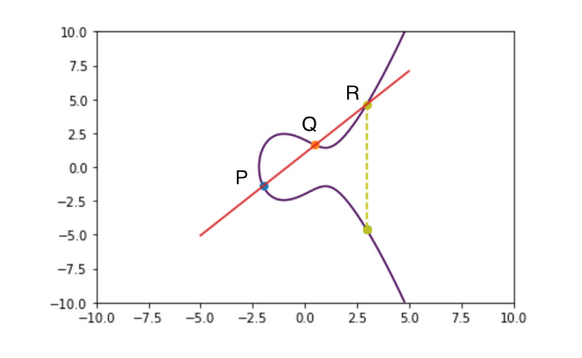
\includegraphics[width=\textwidth]{ECC.png}
	\caption{An elliptic curve. \cite{ECCbasics}}
\end{figure} 

\paragraph{ECDSA} The elliptic curve digital signature algorithm (ECDSA) is the default elliptic curve variant of digital signatures. Like the standard digital signature algorithm (DSA), each signature with length $l$ guarantees a security level of $l/4$(e.g. a signature of 512 bits would guarantee a security level of 128 bits).

\paragraph{ECDH} Besides using ECC for digital signatures with ECDSA, another ECC based protocol that is chosen in this paper is elliptic curve Diffie-Hellman (ECDH). like normal Diffie-Hellman it is used when two communicating parties wish to establish a shared secret (or session key) over an insecure channel. First the two communication parties (Alice and Bob) agree on a base point $G$ and domain parameters $a$ and $b$ of the curve they will use. Second they both generate an ECC key pair: $(P_a,n_a)$ and $(P_b,n_b)$ where $P$ = $nG$ (the base point dotted with itself n times). Third they exchange their public keys $P_a$ and $P_b$. In the last step Alice calculates $S$ = $n_a P_b$ and Bob calculates $S$ = $n_b P_a$. It's important to note that $S$ is the same for both Alice and Bob since $S$ = $n_a P_b$ = $n_a ( n_b G )$ = $n_b ( n_a G )$ = $n_b P_a$. $S$ is the newly created session key that is shared by both parties. Any third party listening on the channel only knows $P_a$ and $P_b$, which are not enough to easily calculate $S$ since they would have to solve the ECDLP.

\paragraph{ECDHE\_ECDSA} As mentioned in section \ref{sec:AK} and illustrated in section \ref{sec:authentication_procedure} it is common practice to combine authentication and shared secret establishment into a single procedure. In \cite{RFC4492} multiple methods are proposed that perform ECDH, while also providing authentication using elliptic curve digital signatures. One of these methods is called ECDHE\_ECDSA and is illustrated in figure \ref{fig:ECDH2}. The extra E in ECDHE comes from th fact that this procedure uses "ephemeral" (i.e temporary) keys. Two communicating parties (Alice and Bob) are both in possession of an elliptic curve private/public key pair: $Pb_a$,$Pr_a$ (Alice) and $Pb_b$,$Pr_b$ (Bob). Alice signals to Bob that she wishes to initiate a ECDHE\_ECDSA sequence by sending a 'hello' message to Bob. Bob then creates a new ephemeral elliptic curve key pair: $Pb_{bE}$,$Pr_{bE}$, signs the new ephemeral public key using his own private key: Sig($Pb_{bE}$,$Pr_b$), and sends this to Alice. She will first verify the signature: Ver(Sig,$Pb_{b}$), thus authenticating Bob to Alice. After which she will also generate her own ephemeral key pair using the same curve as Bob: KGen($Pb_{aE}$,$Pr_{aE}$), before signing the new public key and sending it to Bob: Sig($Pb_{aE}$,$Pr_a$). Bob will then in turn verify the signature using Alice's public key: Ver(Sig,$Pb_{a}$). Alice and Bob are now both in possession resources (e.g. each others ephemeral public keys) to use ECDH to generate a shared secret: $K$=ECDH($Pr_{aE}$,$Pb_{bE}$) for Alice and $K$=ECDH($Pr_{bE}$,$Pb_{aE}$) for Bob. The attentive reader might wonder why these ephemeral key pairs are generated at all. why not use the pre-existing key pairs $Pb_a$,$Pr_a$ and $Pb_b$,$Pr_b$ to generate the shared secret. This is because introducing these ephemeral keys guarantees perfect forward secrecy (PFS)\footnote{Perfect forward secrecy is guaranteed when a posteriori leak of one of the used private keys (e.g. $Pr_a$ and $Pr_b$ in figure \ref{fig:ECDH2}) does not result in the communication session being compromised.}. This is because an attacker in possession of either $Pr_a$ or $Pr_b$ is still not able to obtain the shared secret.


\begin{figure}[h]
	\centering
	\fbox{
		\procedure{ECDHE\_ECDSA}{%
			\textbf{Alice}  \<\< \textbf{Bob} \\
			\text{$Pb_a$,$Pr_a$} \<\< \text{$Pb_b$,$Pr_b$} \\
			\< \sendmessageright{top=\text{hello}} \<\\
			\<\< \text{KGen($Pb_{bE}$,$Pr_{bE}$)} \\
			\< \sendmessageleft{top=\text{Sig($Pb_{bE}$,$Pr_b$)}} \<\\
			\text{Ver(Sig,$Pb_{b}$)} \<\< \\
			\text{KGen($Pb_{aE}$,$Pr_{aE}$)} \<\< \\
			\< \sendmessageright{top=\text{Sig($Pb_{aE}$,$Pr_a$)}} \<\\
			\<\< \text{Ver(Sig,$Pb_{a}$)} \\
			\text{$K$=ECDH($Pr_{aE}$,$Pb_{bE}$)} \<\< \text{$K$=ECDH($Pr_{bE}$,$Pb_{aE}$)} \\
		}
	}
	\caption{ECDHE\_ECDSA}
	\label{fig:ECDH2}
\end{figure} 

\subsubsection{SHA} A lot of cryptographic procedures require the data to be hashed first, and the implementation of this research paper is certainly no exception. The choice was made to use the secure hash algorithm (SHA) family of hash functions. SHA constitutes a large set of cryptographic hash functions that were designed by the United States National Security Institute (NSA). There exist 4 distinct sets of SHA\cite{wiki:SHA}:

\begin{itemize}
	\item \textbf{SHA-0}: Published in 1993, was withdrawn shortly after publication because of a significant flaw.
	
	\item \textbf{SHA-1}: Published in 1995 as a replacement to SHA-0. Has been considered insufficiently secure since 2005.
	
	\item \textbf{SHA-2}: Published in 2001, consists of six hash functions with hash values that are 224, 256, 384 or 512 bits: SHA-224, SHA-256, SHA-384, SHA-512, SHA-512/224, SHA-512/256.
	
	\item \textbf{SHA-3}: Pubished in 2015, subset of the broader cryptographic primitive family Keccak. Conists of the following hash functions: SHA3-224, SHA3-256, SHA3-384 and SHA3-512.
\end{itemize} 
While the SHA-3 hash functions were an obvious candidate, simply because they are newer and deemed more secure, the choice was made to work with the HSA-2 hash functions instead. This is because secure SHA-2 libraries are more readily available for the architecture that was used in our implementation. Another reason is that the MAC function that was chosen also employs SHA-265 as it's cryptographic hash function. 

\subsubsection{HMAC} Once a session key is established between two parties this can be used to authenticate the messages they sent to each other. Since this configuration is symmetric, i.e. they both share the same secret, this is done by using a message authentication code (MAC). The choice was made to work with a hash-based message authentication code (HMAC). HMAC is a specific type of message authentication code (MAC) that uses a cryptographic hash function as well as a secret cryptographic key (in our case the session key established using ECDH). More specifically HMAC-265 (HMAC using SHA-265) was used since it sufficiently secure, as well as there being a library function readily available for our chosen architecture.


\section{Proposed Solution}
\label{sec:solution}

By now, the reader should be familiar with all the key concepts of this paper, as well as why securing the OBD-II is considered a valuable research topic. The following section will be devoted to the solution that was proposed by the researchers of this paper, as well as motivating all design decisions that were made in the process.

\subsection{Role Based Access Control}
\label{sec:sol_RBAC}

They key research question here is: can a solution be developed that would protect an in-vehicle network from unauthorised access via the OBD-II port. The concept of 'unauthorised access' is key, since the goal is not to deny access altogether. Only authorised personnel (e.g. repairmen) should be allowed high levels of access. Meaning that only they should be allowed to start diagnostic sessions, recalibrate ECU's, etc. The only way of differentiating between what is allowed and what isn't is by looking at the messages that are sent, specifically their ID. Some messages, like a message asking for the status of a certain ECU could be considered harmless. The message that is used to initiate a diagnostics session however is not that innocent, since it is shown in \cite{MillerC} that this could be used to disengage the brakes, kill the engine, etc. It follows that any solution to this problem should involve a series of authorisation levels and that each of these is associated with a number of permitted message ID's. The concept of role-based access control (see \ref{sec:RBAC}) is clearly applicable here. Every authorisation level constitutes a role, and what messages are allowed for each level constitute the permissions of this role. More specifically this system should be considered an instance of mandatory access control, since the users are not allowed any control over what permissions they are granted. Now that a system of access control is introduced, we need to look at how this system can be implemented to protect the OBD-II port.

\subsection{Gateway} 
\label{sec:gateway}

The first question to answer is where this system of access control is enforced. A naive implementation would be to introduce and distribute a tool that would connect to the OBD-II port and block/grant access based on some authentication procedure (e.g. entering a code). This approach was taken in \cite{Yadav16}. It was already shown in section \ref{sec:obd_access_control} that this is not a good idea. Mainly because this doesn't stop anyone from circumventing the tool altogether, and connecting to the OBD-II DLC using a custom tool and software. No, it is clear that it shouldn't be possible to gain access to the in-vehicle network via the OBD-II port, circumventing the implemented access control system. We need a component in the vehicle network that is already present and is in charge of all network traffic coming from the OBD-II port. Luckily, this component already exists in most in-vehicle networks. It is called the gateway ECU. Originally this component is introduced to have seamless communication between different networks in a vehicle. But as was discussed in section \ref{sec:vni} it is also in charge of translating and forwarding messages coming from the OBD-II port. Every message coming from the OBD-II must pass through this component. This makes the gateway the ideal location to enforce OBD-II access control. 

\subsection{Symmetric/Asymmetric Keys} 
\label{sec:symmetric/asymmetric_keys}

Now that an appropriate location is selected let's look at the access control system itself. In a common enterprise RBAC system the worker authenticates to the system via a password, key-card, retinal scan, etc. The common theme of all these methods is the possession of some type of authentication key. The worker authenticates to the system by proving he/she is in possession of the appropriate key. Translating this concept to our situation the user (e.g. car owner, repairman, policeman, etc) authenticates him-or-herself by proving to the system (the gateway of the vehicle) that he or she is in possession of the appropriate key. The choice was made to make use of cryptographic keys to implement access control as well as associating a different security policy (and by extension different keys) for every car model. From section \ref{sec:PKC} it follows that there are two cryptographic key configurations that can be considered: symmetric and asymmetric. symmetric cryptography has the advantage of shorter key lengths, however this would entail that if the keys of one vehicle were extracted (e.g. by extracting and analysing the gateway) and distributed, all vehicles of the same model would be compromised. That is why the decision was made to use asymmetric keys, but in what configuration? The first option is for the gateway to hold the private keys, whereas the users are in possession of the appropriate public keys. However, This configuration has the same major design flaw that symmetric encryption had, namely possible extraction of the private key from the vehicle. The configuration that remains, and which is the one chosen by the researchers of this paper, is to distribute the private keys to the users, while storing the public keys inside the gateway. More specifically it was chosen to use elliptic curve public keys, since they provide more efficient operations than other public key techniques (see section \ref{sec:ECC} for more information on elliptic curves). The decision to use asymmetric keys moves the responsibility of safely storing the private key to the users. Intuitively this might seem worse, since now the private keys are already in the hands of individuals. Individuals that might have ulterior motives concerning their level of access. However, this concern can be countered by noting that ideally these individuals would not be directly in possession of the private key. In a world where the internet is ubiquitous, it is not hard to conceive of a device that handles the authentication procedure with the gateway (called the tester in this paper). Thereby connecting to a central server where the private keys are actually stored. This concept will become clear when the authentication protocol is discussed.

\subsection{Authentication Procedure}
\label{sec:authentication_procedure}

The next step is to define the authentication procedure itself, i.e. how does a user prove to the gateway that he or she is in possession of the appropriate private key. A couple of attempts were proposed throughout the course of our research. The first attempt is to periodically complete a challenge-handshake authentication protocol (CHAP). The second is the complete a CHAP, followed by establishing a secret key. The third and final attempt is to combine authentication and shared secret establishment into one procedure.

\subsubsection{Attempt 1: CHAP} Using the challenge-handshake authentication protocol the gateway would send a challenge (which is randomly generated) to the tester\footnote{In the remainder of this paper we'll be referring to the device the user uses to authenticate to the OBD-II interface as the tester.}. The tester would sign this challenge using the appropriate private key, and return this signature to the gateway. The gateway can then verify the correctness of this signature using the appropriate public key. The problem is that this procedure would have to repeated periodically to ensure the authenticated session isn't hijacked, i.e. the authenticated user has disconnected and another unauthorised user is now sending messages to the network. Concerning the length of this period, there are 2 extreme options, both motivated by opposing concerns:

\begin{itemize}
	\item \textbf{Smallest Possible Period:} This option is motivated by the fact that having a very small period (i.e. initiating a CHAP before every message) would improve the overall security of the system. Indeed, any message forwarded on the bus was preceded by a CHAP.
	
	\item \textbf{Largest Possible Period:} This option is motivated by the fact that public key operations are computationally complex, resulting in slower algorithms. Having a large period would minimize the amount of cryptographic operations (i.e. signing) being performed, improving the efficiency of the system.	
\end{itemize}

It is clear that the ideal solution would lie somewhere in the middle, allowing for a smooth operation while still guaranteeing a sufficient level of security. However, this problem can be circumvented altogether by taking a very different approach: instead of repeatedly initiating a CHAP, we could authenticate, then establish a shared secret, and afterwards each message would be authenticated using this shared secret. This approach is discussed next.

\subsubsection{Attempt 2: CHAP + ECDH}
Since it was chosen to use elliptic curve public/private key pairs, It should come as no surprise that elliptic curve Diffie-Hellman (ECDH) is considered as our secret key exchange mechanism (for more information on ECDH see section \ref{sec:ECC}). To authenticate to the gateway, the tester would first authenticate (by completing a CHAP), then establish a shared secret, and afterwards this shared secret would be used to authenticate every single message. The attentive reader might notice a significant flaw with this approach. Namely, that an attacker could hijack the system after the first step (i.e. completing the CHAP), establishing their own shared secret with the gateway, thereby being granted unauthorised access to the in-vehicle network. The problem here is that the authentication procedure (CHAP) is separated from the key exchange procedure (ECDH). Ideally, these procedures should be combined, forming a single procedure that succeeds in authenticating the tester to the gateway, while also safely exchanging a secret key to use in the upcoming communications session. 

\subsubsection{Attempt 3: ECDHE\_ECDSA} 
In the third and final attempt we start from the ECDHE\_ECDSA algorithm introduced in section \ref{sec:ECC}, more specifically figure \ref{fig:ECDH2}. This algorithm does exactly what is desired: combine authentication with shared secret establishment. A couple of changes to this algorithm can be applied to more closely adhere to our situation:
\begin{enumerate}
	\item \textbf{Gateway Key Pair:} A precondition for the ECDHE\_ECDSA algorithm is that both parties have an ECC key pair already established. For the tester this condition is already met. Even better, the corresponding public key is already given to the gateway. For the gateway however this is not the case. Since ECDH requires two key pairs, a new key pair will have to computed every time the procedure is run.
	
	\item \textbf{Perfect Forward Secrecy:} We can get rid of the ephemeral keys. This is because perfect forward secrecy (or secrecy in general) is not a goal in our situation. the goal is to protect against unauthorised access, not to protect past sessions from leaking. 
	
	\item \textbf{Mutual Authentication:} The first authentication step can be omitted (i.e signing by the gateway, and verification by the tester). Because of the absence of a gateway key pair, it is impossible for the gateway to authenticate itself to the tester. Moreover, this is not even a requirement of our authentication procedure.
\end{enumerate}
Applying all of these modifications the procedure from figure \ref{fig:authentication_procedure} is obtained. Before the procedure is initiated the tester is in possession of the OBD-II private key $Pr_{obd}$ while the gateway has the appropriate public key $Pb_{obd}$ stored in memory. The user of the tester initiates the procedure by connecting to the OBD-II DLC, after which the tester sends an initialization message to the gateway. This initialization message also specifies the role that the user of the tester wishes to authenticate as. The gateway responds to this by creating a new ECC key pair: KGen($Pb_g$,$Pr_g$), and sending the newly created public key ($Pb_g$) to the tester. The tester then signs this public key using the OBD-II private key and sends this signature (only the signature) back to the gateway: Sig($Pb_g$,$Pr_obd$). After the gateway has verified the signature using the OBD-II private key: Ver(Sig,$Pb_{obd}$), both parties calculate the shared secret using ECDH: $K$=ECDH($Pr_{obd}$,$Pb_g$) for the tester and $K$=ECDH($Pr_g$,$Pb_{obd}$) for the gateway. This newly created secret can then be used to authenticate every OBD-II message that is sent in the upcoming session.
 
\begin{figure}[h]
	\centering
	\fbox{
		\procedure{OBD-II Authentication Procedure}{%
			\textbf{Tester}  \<\< \textbf{Gateway} \\
			\text{$Pr_{obd}$} \<\< \text{$Pb_{obd}$} \\
			\< \sendmessageright{top=\text{init}} \<\\
			\<\< \text{KGen($Pb_g$,$Pr_g$)} \\
			\< \sendmessageleft{top=\text{$Pb_g$}} \<\\
			\< \sendmessageright{top=\text{Sig($Pb_g$,$Pr_obd$)}} \<\\
			\<\< \text{Ver(Sig,$Pb_{obd}$)} \\
			\text{$K$=ECDH($Pr_{obd}$,$Pb_g$)} \<\< \text{$K$=ECDH($Pr_g$,$Pb_{obd}$)} \\
		}
	}
	\caption{OBD-II Authentication Procedure}
	\label{fig:authentication_procedure}
\end{figure}

\subsection{Private Key Storage} It is important to address an issue that was posed earlier in section \ref{sec:symmetric/asymmetric_keys}, namely how to protect against the private keys being leaked? The obvious solution is to store them in protected memory on the tester. Making it hard for them to be extracted via reverse engineering or side-channel attacks. However, a more elegant solution presents itself: If the tester device were to be connected to the internet, it could forward the public key it receives from the gateway to a central server. This central server (where the private keys are securely stored) could then sign the public key, and send back the signature to the tester, which will in turn use it to continue the authentication procedure. This way the private keys are never distributed, decreasing the chance of them ever leaking. 

\subsection{Message Authentication}
The authentication procedure from section \ref{sec:authentication_procedure} authenticates the tester to the gateway, thereby also establishing a shared secret. The next step is to design a procedure that uses this shared secret to facilitate an authenticated communications session. The solution proposed by the researchers of this paper is simple and illustrated in figure \ref{fig:message_authentication}. The OBD-II message sent by the tester ($M$) is followed up by a message containing a MAC: MAC($M$,$K$) (see section \ref{sec:MAC}). This MAC is calculated by inputting the data of the first CAN frame as well as the recently established secret key $K$. Before the gateway forwards the message to the appropriate sub-network, it first performs two distinct security checks: 
\begin{itemize}
	\item \textbf{Permissions Check} CheckP($M$): This is where the role based access control system proposed in section \ref{sec:sol_RBAC} is actually enforced. The gateway knows what role the tester authenticated as, so the first condition that is checked is whether this role has permission to send the message $M$. It will do this this by looking up the ID of the message in the permissions table (see section \ref{sec:permissions_table}). If the message ID is not present, the message will be denied and the tester (and by extension the user) is notified.
	
	\item \textbf{MAC Verification} Ver(MAC,$K$): After the message $M$ passes the permissions check, the gateway will check whether the received MAC is correct. This way ensuring that the sender of this message is authorized. Again, if this test fails the message will be denied and the tester is notified
\end{itemize}
If both these checks succeed, the OBD-II message $M$ is forwarded to the appropriate sub-network and the tester receives an acknowledgement (ACK). The order of the two checking operations is motivated by the fact that the MAC verification operation takes much longer to perform than checking the permissions table. By checking the permissions first, it is avoided that a previously initiated signature verification operation is rendered redundant (e.g. when the permissions check fails).

\begin{figure}[h]
	\centering
	\fbox{
		\procedure{Message Authentication}{%
			\textbf{Tester}  \<\< \textbf{Gateway} \<\< \textbf{Network}\\
			\text{$K$}  \<\< \text{$K$} \<\< \\
			\< \sendmessageright{top=\text{OBD-II message $M$}} \<\<\<\\
			\< \sendmessageright{top=\text{MAC($M$,$K$)}} \<\<\<\\
			\<\< \text{CheckP($M$)} \<\< \\
			\<\< \text{Ver(MAC,$K$)} \<\< \\
			\<\<\< \sendmessageright{top=\text{$M$}} \< \\
			\< \sendmessageleft{top=\text{ACK}} \<\<\< \\
		}
	}
	\caption{OBD-II Message Authentication}
	\label{fig:message_authentication}
\end{figure}

\subsection{Permissions Table} 
\label{sec:permissions_table}
The permissions table is stored on the gateway, and is used to determine which OBD-II messages are allowed for each role.

\backmatter

\bibliographystyle{plainurl}
\bibliography{references}

\end{document}

